% Created 2018-10-07 Sun 23:58
% Intended LaTeX compiler: pdflatex
\documentclass[11pt]{article}
\usepackage[utf8]{inputenc}
\usepackage[T1]{fontenc}
\usepackage{graphicx}
\usepackage{grffile}
\usepackage{longtable}
\usepackage{wrapfig}
\usepackage{rotating}
\usepackage[normalem]{ulem}
\usepackage{amsmath}
\usepackage{textcomp}
\usepackage{amssymb}
\usepackage{capt-of}
\usepackage{hyperref}
\author{Kevin Poli}
\date{\today}
\title{}
\hypersetup{
 pdfauthor={Kevin Poli},
 pdftitle={},
 pdfkeywords={},
 pdfsubject={},
 pdfcreator={Emacs 26.1 (Org mode 9.1.14)}, 
 pdflang={English}}
\begin{document}

\tableofcontents

\section{Telescope}
\label{sec:org08d2e3a}
Kevin Poli, Phil Vitale, Connor O'Hara and Brendan Von Hofe
\section{Intro}
\label{sec:orgdd20d79}
Telescope is a machine learning assisted toolkit for digital video compositors
with applications in visual effects, matte painting and diverse use cases
accross the video post production pipeline. Tools from existing compositing
packages will interact with a novel ML core to assist or completely automate the
rotoscoping process. Rotoscoping is the process of masking and segmenting
poritons of an image accross multiple moving frames, any feature length movie
will often consist of hundreds of rotoscoped shots with multiple tracked mattes
per image, and this is the primary job of thousands of roto artists accross the world.

We hope to make this process, fast, intuitive, and accesible to alleviate the
manual and time consuming process that makes up a huge chunk of the man hours
required to produce even low budget features. We believe that machine learning
is in the process of revolutionizing image processing, and that user driven
toolkits rather than black box command line workflows will bring our intelligent
core into the hands of the artists where they can thrive.
\subsection{Demonstration}
\label{sec:org44dcadf}
Rotoscoping is the process of frame by frame selecting and isolating a given feature (usually
an object or person) in a video, such that you can produce a video clip of
exclusively that selection on a transparent background

Lets walk through this step by step:

\begin{itemize}
\item First, our source image at frame 1, of Marceu the Mime
\begin{center}
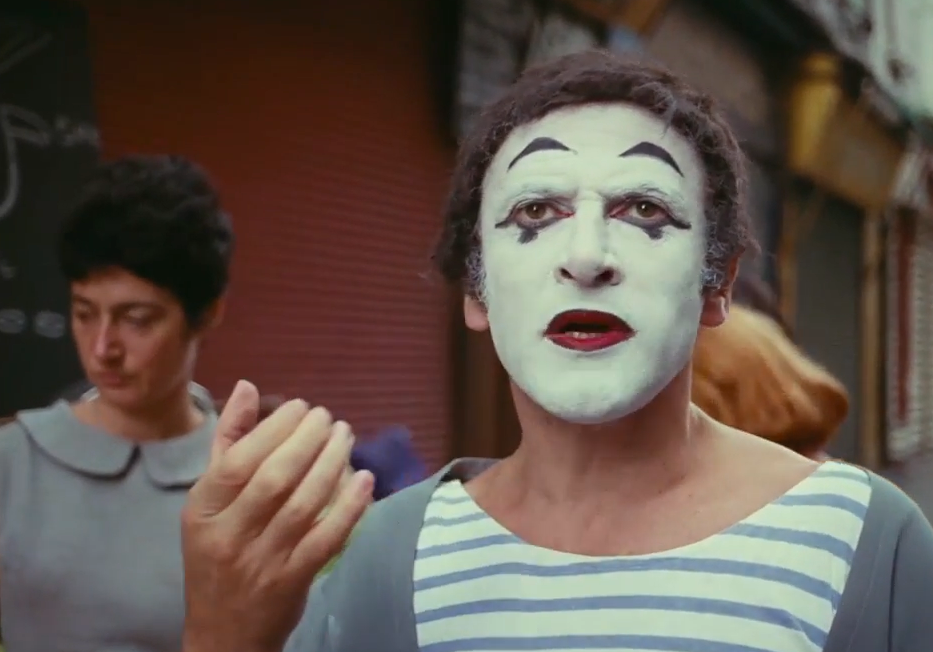
\includegraphics[width=.9\linewidth]{./roto/Capture.PNG}
\end{center}
\item Lets start by creating a selection just of the Mime's face and hand - these
are the features that are actually being "rotoscoped" out
\begin{center}
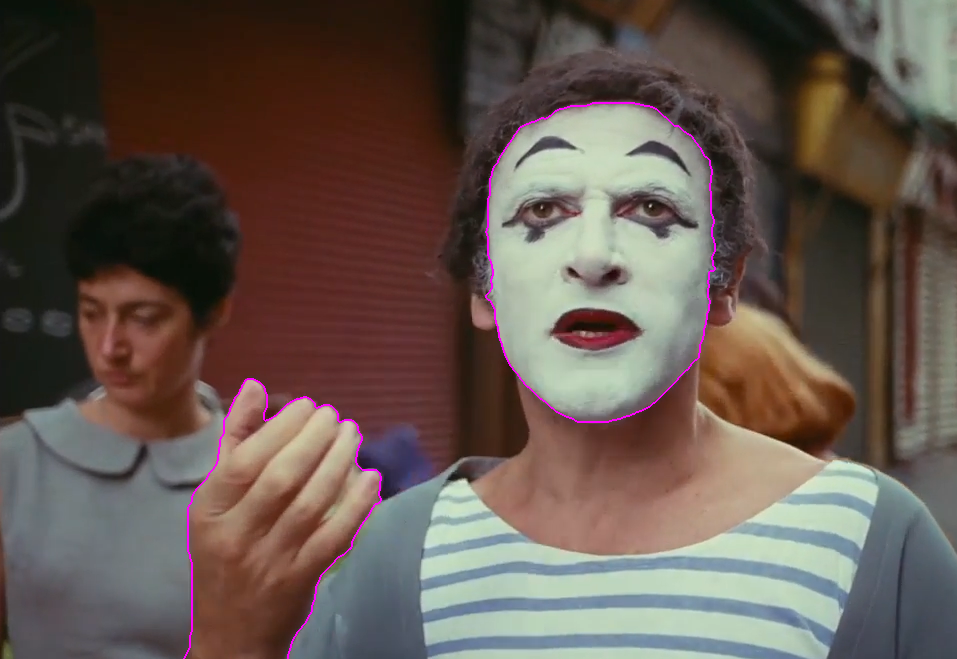
\includegraphics[width=.9\linewidth]{./roto/masked.PNG}
\end{center}
\item This purple selection represents a 'mask' which are the points and curves that
make up the boundary of what we are looking to isolate. Traditionally, artists
will digitally paint this selection in a software of their choice, by hand.
\item This selection or mask is different from a matte, which is another important
piece of terminology. A matte is a single channel image; meaning rather than
pixels having red,green,blue values, they only contain 1 value from 0-255
called 'alpha'. 'Alpha' will often be displayed in software as white. The
Matte of this selection is an image where only the pixels corresponding to the
selection are white, and all other pixels are black.
\begin{center}

\includegraphics[width=.9\linewidth]{./roto/matte.PNG}
\end{center}
\begin{itemize}
\item this is so that, under the hood, all we need to do is pixel-wise 'multiply' the
source image to the matte, meaning any pixels with a black 'zero value' in
the matte will become transparent, and any pixels in the white '255 value'
in the matte will remain.
\end{itemize}
\begin{center}
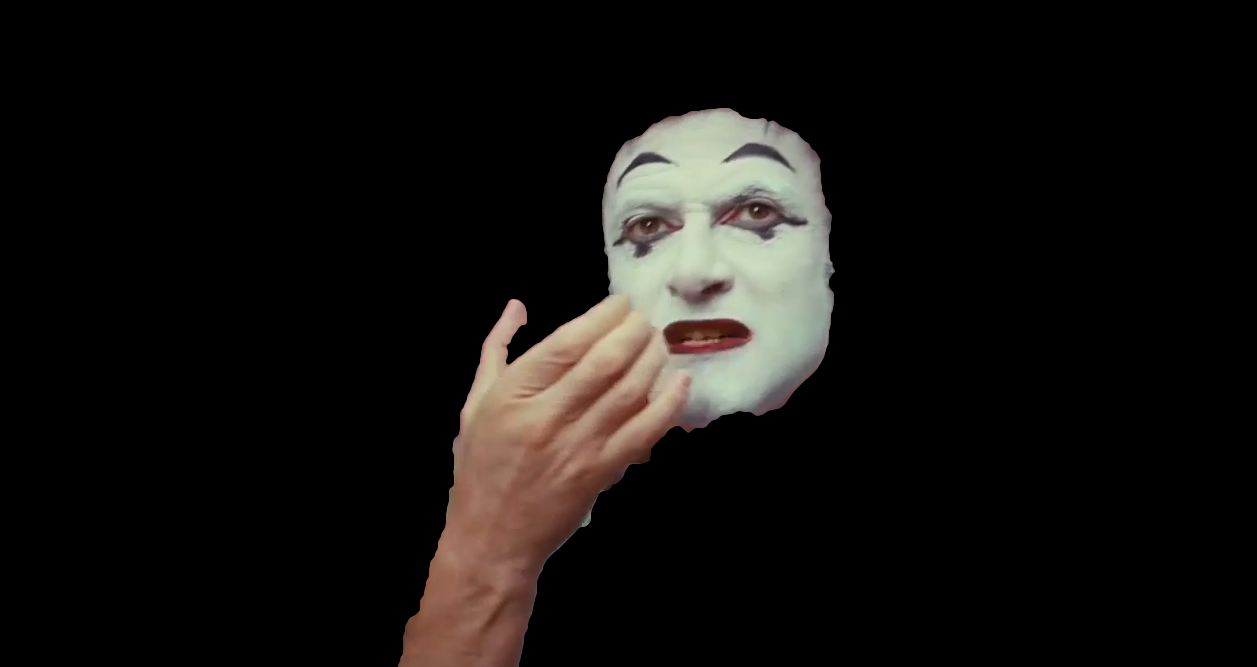
\includegraphics[width=.9\linewidth]{./roto/goals.PNG}
\end{center}
\begin{itemize}
\item Here is the result of that multiply, an image containing only the pixels we
selected before
\end{itemize}
\end{itemize}
\subsubsection{Frame By Frame}
\label{sec:org2723b87}
Much of the challenge and tedium of rotoscoping comes from repeating the above
process for every frame, traditionally, artists will go frame by frame through
the video and manually adjust their selections to match the feature they are
isolating, here is the next frame of that video, with an adjusted selection for
clarity

\begin{center}
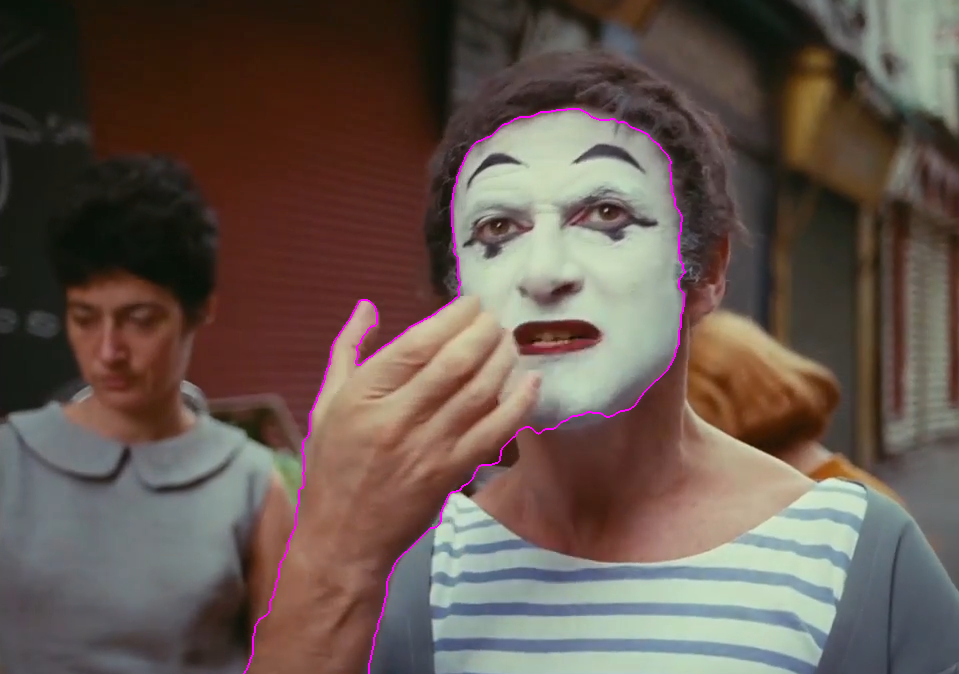
\includegraphics[width=.9\linewidth]{./roto/nextframe.PNG}
\end{center}
\subsubsection{Use Cases}
\label{sec:orge055300}
With our selection isolated, we can start to play with the image accordingly

By layering the source footage and our rotoscoped hand and face, we can apply an
effect, like the 'colorama' effect to only the pixels we roto'd previously

\begin{center}
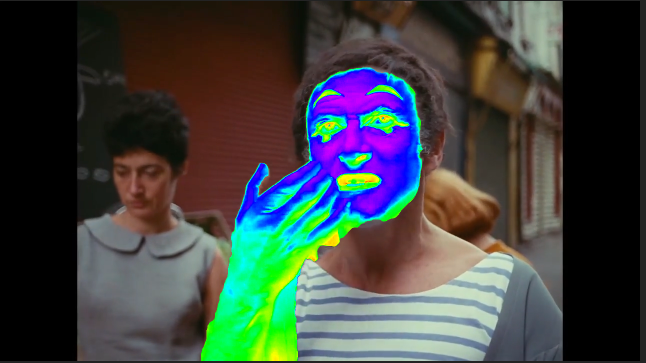
\includegraphics[width=.9\linewidth]{./roto/isolated.PNG}
\end{center}
\begin{enumerate}
\item Compositing
\label{sec:org3873182}
The most popular use case for rotoscoping is Compositing, which is the process
of combining multiple images into one. Consider three layers to see how this is
done.

Say we want this red square video clip to appear 'behind' the Mime's face and
hand (note what appears black is acutally transparent)

\begin{center}

\includegraphics[width=.9\linewidth]{./roto/red.PNG}
\end{center}

We can grab our source clip and place the square image on top
  \begin{center}
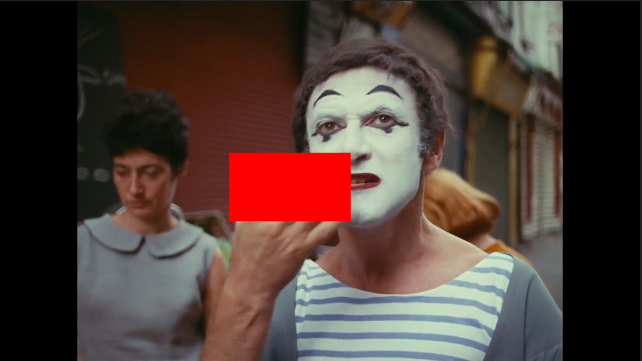
\includegraphics[width=.9\linewidth]{./roto/halfcomp.PNG}
\end{center}
Then grab our rotoscoped face and hand and place that on top
  \begin{center}
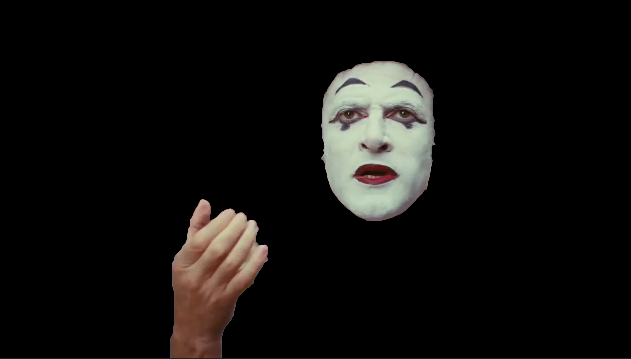
\includegraphics[width=.9\linewidth]{./roto/void.PNG}
\end{center}
And place it on top for the desired effect

\begin{center}
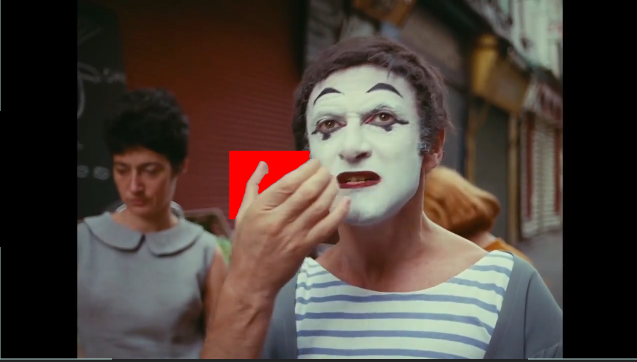
\includegraphics[width=.9\linewidth]{./roto/behind.PNG}
\end{center}
\end{enumerate}
\section{Technical Plan}
\label{sec:org5c42796}
\subsection{Components}
\label{sec:org239a824}
Telescope as a product will consist of two primary modules, the Telescope Core,
which is a machine learning core assisted by traditional algorithmics that
implements the novel functionality of Telescope, and an exchange plugin that
allows existing professional compositing tools to interact with our proccesses.
Telescope For Nuke is our chosen example exhange plugin, designed to demonstrate
how the Telescope core can interact with existing artist workflows - but the
separation of core and plugin is designed such that Telescope can be implemented
into other software packages like Adobe After Effects or Blackmagic Design
Fusion at a later date.

\begin{center}
\begin{tabular}{ll}
Category & What are we using?\\
\hline
Communication & \\
Email & Gmail\\
Web Conferencing & Facebook Video\\
Instant Messaging & GroupMe\\
Collaboration & \\
Document Collaboration & Google Drive\\
File Sharing/Data Tracking & GitHub\\
Plugin Development & \\
OS Supported & Windows, Mac OS, Linux\\
Host Application & Nuke\\
Development Language & C++\\
Machine Learning Development & \\
Development Language & Python\\
Packages & PyTorch\\
\end{tabular}
\end{center}
\subsection{Algorithmics}
\label{sec:org08ca268}

The algorithmic core of our plugin will take images (frames of videos) as input and output segmentation masks (mattes) as output. The goal of the masks is to identify all the discrete objects in the image. It is class-agnostic and therefore does not need to determine what the objects are (e.g. cat or dog) but rather the fact that they are discrete.
Our criteria for determining how well our model is accomplishing the task is the Intersection-over-Union metric (IoU). We have yet to determine what an acceptable IoU score is for industry applications.
The model will be a convolutional neural network. Specifically, we will begin with the UNet model (\url{https://arxiv.org/abs/1505.04597}). Initially, our primary dataset to train the model with will be the Panoptic Detection COCO dataset, modified for a class-agnostic task.
Further iterations of the model will take advantage of the additional information in EXR images to refine object mattes and the DAVIS video object segmentation dataset.

\subsection{Dependency Model}
\label{sec:org04cf880}
\begin{center}
\includesvg[width=.9\linewidth]{./DGraph}
\end{center}



\section{Team}
\label{sec:orgd19d869}
\subsection{Roles}
\label{sec:org4726946}
\begin{itemize}
\item Connor O’Hara: Image Processing (cohara1@stevens.edu)
\item Kevin Poli: Application/ Artist Tools Developer (kpoli@stevens.edu)
\item Philip Vitale: Application \& Systems Developer (pvitale@stevens.edu)
\item Brendan von Hofe: Machine Learning (bvonhofe@stevens.edu)
\end{itemize}

Advisors: Hong Man (hman@stevens.edu), Jeff Thompson (JThomps4@stevens.edu)


\subsection{Delegation of Tasks}
\label{sec:orge8e8cad}

\textbf{Connor O’Hara}
\subsubsection{Last Week}
\label{sec:org5d1663a}
\begin{itemize}
\item Continue contact with Venture Center
\begin{itemize}
\item we have a primary contact, but still waiting to be met with
\end{itemize}
\end{itemize}
\subsubsection{This week}
\label{sec:org90d9eae}
\begin{itemize}
\item Research Generative Ladder Networks
\end{itemize}


\textbf{Kevin Poli}
\subsubsection{Last Week}
\label{sec:orgaa0c34c}
\begin{itemize}
\item Acquire developer license for Nuke
\begin{itemize}
\item Working on trial version until license is acquired
\end{itemize}
\end{itemize}
\subsubsection{This week}
\label{sec:orgb708ebc}
\begin{itemize}
\item Follow along with Nuke developer tutorials, implement Nuke boilerplate
\end{itemize}

\textbf{Philip Vitale}
\subsubsection{Last week}
\label{sec:org3c0adeb}
\begin{itemize}
\item Nuke API research
\begin{itemize}
\item Noted and shared video tutorials and downloaded the manual
\end{itemize}
\end{itemize}
\subsubsection{This week}
\label{sec:org4a4f2e7}
\begin{itemize}
\item Follow along with Nuke developer tutorials, implement Nuke boilerplate
\end{itemize}
\textbf{Brendan Von Hofe}
\subsubsection{Last Week}
\label{sec:org4971971}
\begin{itemize}
\item Define image processing model
\end{itemize}
\subsubsection{This Week}
\label{sec:orga3b66d3}
\begin{itemize}
\item Researching how to improve older partial solutions DeepMask/SharpMask
\item \url{https://github.com/facebookresearch/deepmask}
\end{itemize}

Team  
\subsubsection{Updates}
\label{sec:org9bb0323}
\begin{itemize}
\item Meet with Visual Arts department
\begin{itemize}
\item Move forward taking them on as our client, Hong Man will remain Advisor
\end{itemize}
\item Attend tech meetup for capital/business opportunity
\begin{itemize}
\item Machine learning meetup October 4th
\end{itemize}
\end{itemize}
\end{document}
